
%\documentclass[letterpaper, 10 pt, conference]{ieeeconf}  % Comment this line out if you need a4paper

\documentclass[a4paper, 10pt, conference]{ieeeconf}      % Use this line for a4 paper

\IEEEoverridecommandlockouts                              % This command is only needed if 
                                                          % you want to use the \thanks command
\overrideIEEEmargins                                      % Needed to meet printer requirements.

% See the \addtolength command later in the file to balance the column lengths
% on the last page of the document

% The following packages can be found on http:\\www.ctan.org
\usepackage{graphicx} % for pdf, bitmapped graphics files
\usepackage{epsfig} % for postscript graphics files
%\usepackage{mathptmx} % assumes new font selection scheme installed
%\usepackage{times} % assumes new font selection scheme installed
\usepackage{amsmath} % assumes amsmath package installed
%\usepackage{amssymb}  % assumes amsmath package installed

%%%%%CUSTOM%%%%%

\usepackage{alltt}
\usepackage[usenames,dvipsnames]{xcolor}
\usepackage{xytree}
\usepackage{tikz-dependency}
\usepackage{pict2e}

\DeclareMathOperator*{\argmax}{arg\,max}
\renewcommand*\sfdefault{ppl}

\usepackage{pgf}
\usepackage{tikz}
\usetikzlibrary{arrows,automata,shapes}

\usepackage{float}

\usepackage[algoruled,vlined]{algorithm2e}



%%%END CUSTOM%%%

\title{\LARGE \bf
Controlled Natural Languages in Artificial Cognition:\\ Language Generation and Action Formalization
}
\author{Nicholas H. Kirk$^{1}$, Daniel Nyga$^{1,2}$, Michael Beetz$^{2}$\\
$^{1}$Intelligent Autonomous Systems, Technische Universit\"{a}t M\"{u}nchen, Germany\\
$^{2}$Institute for Artificial Intelligence \& TZI\footnote{The Center for Computing Technologies (TZI)}, University of Bremen, Germany\\
{\sffamily {nicholas.kirk@tum.de}, {nyga@cs.tum.edu}, {beetz@cs.uni-bremen.de}}\\
%\institute{$^1$Intelligent Autonomous Systems, Technische Universit�t M�nchen, Germany\\
%$^2$Institute for Artificial Intelligence \& TZI\footnote{The Center for Computing Technologies (TZI)}, University of Bremen, Germany}
%\email{nicholas.kirk@tum.de}, \email{nyga@cs.tum.edu}, \email{beetz@cs.uni-bremen.de}
}

% \thanks{*This work was not supported by any organization}% <-this % stops a space
% \thanks{$^{1}$Albert Author is with Faculty of Electrical Engineering, Mathematics and Computer Science,
%         University of Twente, 7500 AE Enschede, The Netherlands
%         {\tt\small albert.author@papercept.net}}%
% \thanks{$^{2}$Bernard D. Researcheris with the Department of Electrical Engineering, Wright State University,
%         Dayton, OH 45435, USA
%         {\tt\small b.d.researcher@ieee.org}}%
%

\begin{document}

\maketitle
\thispagestyle{empty}
\pagestyle{empty}

%%%%%%%%%%%%%%%%%%%%%%%%%%%%%%%%%%%%%%%%%%%%%%%%%%%%%%%%%%%%%%%%%%%%%%%%%%%%%%%%
\begin{abstract}
In this paper we discuss, within the context of artificial assistants
 performing everyday activities, a resolution method to disambiguate 
 missing or not satisfactorily inferred action-specific information 
 via explicit clarification.
While arguing the lack of preexisting human-robot interaction means, 
we introduce novel uses of Controlled Natural Languages (CNL)
as means of linguistic human-robot interaction and action-oriented 
representation formalization.\\
We additionally provide implemented working scenarios, 
state future possibilities and problems related to formalization 
of technical cognition.
\end{abstract}

%%%%%%%%%%%%%%%%%%%%%%%%%%%%%%%%%%%%%%%%%%%%%%%%%%%%%%%%%%%%%%%%%%%%%%%%%%%%%%%%
\section{Introduction}

In everyday routine activities, robotic assistants and co-workers 
will have to perform a variety of tasks for which they cannot be 
pre-programmed because they are not known at production time. 
Research in the field of cognitive robotics envisions service 
robots that autonomously acquire new skills and adapt existing ones 
to new tasks and environments. They must decide on \textit{how} to 
perform a particular activity at runtime, which requires them to infer 
the \textit{appropriate} actions to be executed on the \textit 
{appropriate} objects in an \textit{appropriate} way. They have to 
perform what is commonly referred to as \textit{everyday activity}, 
which has been proven to be a very knowledge-intensive task~\cite 
{anderson95phd, nyga12actioncore}. It requires context awareness and 
flexibility in action parametrization when operating in real world 
settings with partially available data, which is referred to as the 
``open world challenge.'' 

Recent research in the field of cognitive robotics aims to make 
knowledge sources available for robots, which have been created by 
humans and are intended for human use. For some domains such as 
daily household tasks (e.g. cooking or cleaning up), step-by-step 
plans and recipes from web pages like \textit 
{wikihow.com} have been successfully used for feeding such common 
sense knowledge about actions and objects into knowledge bases of 
mobile robotic platforms and for transforming such recipes into 
executable robot plans~\cite{tenorth10webinstructions}. 

However, as these recipes are presented in natural language, severe ambiguity, 
vagueness and underspecification have been identified as major 
challenges in translating into plans, since many missing 
key pieces of information are generally considered common sense to 
\begin{figure}[t]
%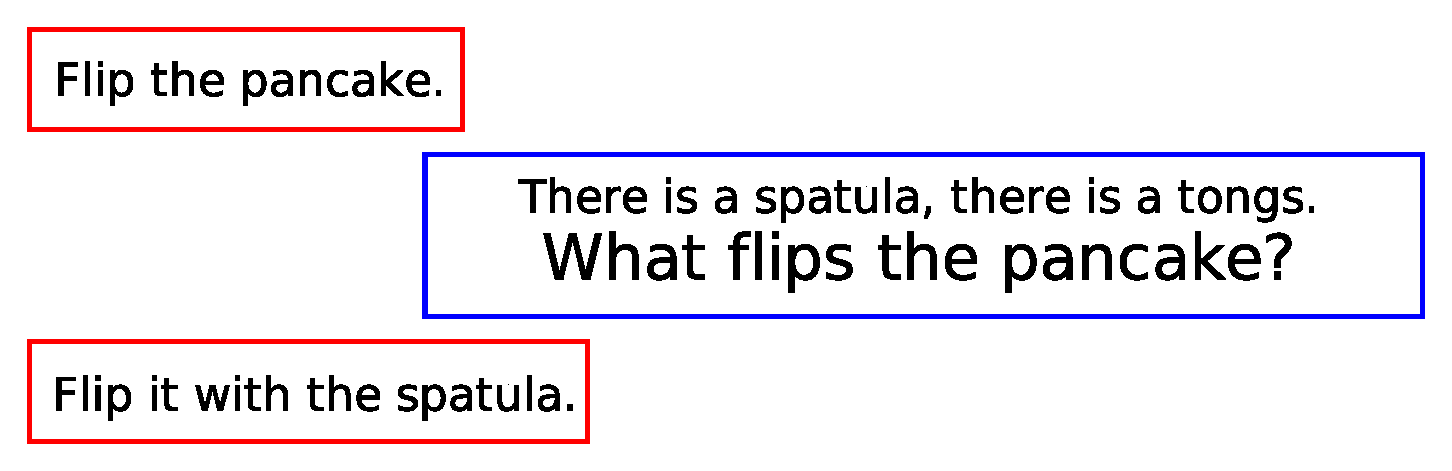
\includegraphics[width=.9\columnwidth]{introduction.eps}
\centering
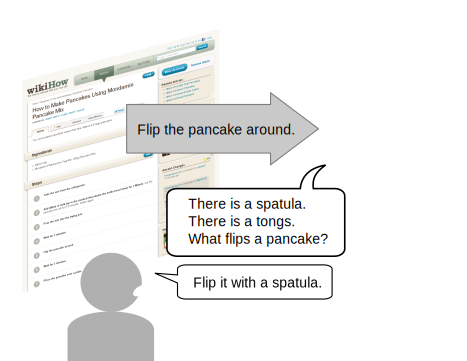
\includegraphics[scale=0.65, trim = 0mm 0mm 0mm 8mm]{human_robot.pdf}
\caption{Representation of a disambiguation interaction}
\label{fig:application}
\end{figure} 
the human, making these unserviceable.
%and hence explicit statements of these kinds of 
%self-evident yet necessary information are rendered inefficient. 
As an example, consider the natural-language instruction ``Flip the 
pancake'', taken from a recipe for making pancakes: 
In order to perform the action successfully, a robot needs to decide 
which utensil to use (e.g. a spatula), where to hold it (e.g. at its 
handle) and what part of it to put underneath the pancake (e.g. the 
blade), to name only a few.
Current research in cognitive robotics aims to build action 
verb-specific knowledge bases that fill these knowledge gaps and 
enables a robot to infer the information which is \textit{needed} in 
order to perform a particular activity, based on what is \textit 
{given} in a naturalistic action specification.

However, such inference might be insufficient to formulate action 
specification and require the robot to fall back on human assistance. 
As an example, consider a situation where 
the robot is asked to flip a pancake, but the knowledge base does 
not contain sufficient information about what instrument is to be used 
(e.g. it has no strong preference for a spatula over barbecue 
tongs). In such a case, the robot has to explicitly ask a human for 
instrument clarification. Figure \ref{fig:application} illustrates such a 
situation. Taxonomical and compositional relationships, object role 
understanding, are only some of the missing elements that could 
potentially require clarification. 

%In this work, we present an implementation of a novel approach for 
%identifying and verbalizing such absent information in a knowledge
% base, in order to enable a robot to actively enhance its knowledge
%  about actions and objects by stepping into dialog with humans.
  
In this work, we present an implementation of a novel dialog-based approach that enables robots to 
identify such knowledge gaps, ask for clarification and integrate replies. 
   
The contributions of this paper, within the artificial cognition domain,
 are the following:
\begin{enumerate}
    \item CNL as means of language generation \hfill [implemented]
    \item CNL as means of action-oriented formalization \hfill [work in progress]
\end{enumerate}
The remainder of this paper is organized as follows: 
description of the adopted technologies (\textit{PRAC, ACE, DRS}), 
explanation of how the claims are related to the state of the art, 
explanation of the implemented language generation module and of the current work
 in progress towards full action formalization. Last but not least, 
 an ending summary comprising results, current limitations and future perspectives is presented.

\section{Adopted Technologies}
\subsection{Probabilistic Robot Action Cores}

Nyga et al.\cite{nyga12actioncore} introduced the concept of 
\emph{Probabilistic Robot Action Cores} (PRAC), which can be thought as abstract,
generic event patterns representing sets of 
inter- and intraconceptual relations that constitute an abstract 
event type, assigning an action role to each entity that is affected 
by the respective action verb. Formally, a PRAC is defined as a conditional
probability distribution:

{\large
\begin{equation}
P\left(\mathcal{R}\times\mathcal{A}\times\mathcal{C}\,|\,\sqsubseteq
,\, \preceq \right) \enspace . \label{pracformula}
\end{equation}
}
{\small
\begin{center} \begin{tabular}{ll}
    $\mathcal{R}$  & is the set of all action roles\\
    $\mathcal{A}$  & is the set of all action verbs\\
    $\mathcal{C}$  & is the set of all class concepts\\
    %$P$ &  \text{is a probability distribution}\\
	%&  \text{over all role assignments of an action}\\
    %$\pi$ &  $\pi:\mathcal{A}\rightarrow 2^{\mathcal{R}}$ \text{ is a function that selects}\\
    %& \text{the needed roles given an action}\\
    $\sqsubseteq$ & is a taxonomy relation over $\mathcal{C}$\\
    $\preceq$	& is a mereological relation over $\mathcal{C}$
\end{tabular}
\end{center}}
As opposed to most approaches towards understanding natural-language 
instructions, which merely seek to understand what is given by an 
instruction, the PRAC concept is also able to infer what is missing. 
It combines action-specific and ontological world knowledge in a 
joint probabilistic first-order representation, which allows to 
automatically find generalizations from concrete event occurrences 
at an appropriate level of abstraction. Specifically, PRAC models 
are represented as a set of action roles (objects involved in the 
action with a specific role) and Markov Logic Networks (MLN), a 
knowledge representation formalism that combines first-order logic 
and probability theory~\cite{DBLP:journals/ml/RichardsonD06}. In this
work, we use the definitions of Action Roles in order to identify and
verbalize insufficient information about action parameterization. For a 
detailed definition of PRAC Action Cores and Roles, we refer to \cite{nyga12actioncore}.

\begin{figure}[H]
{\sffamily
\begin{itemize}
    \item \textit{Action Core:} Flipping
    \item \textit{Definition:} An Agent causes a Theme to move with respect to a FixedLocation, 
generally with a certain Periodicity, without undergoing unbounded translational 
motion or significant alteration of configuration/shape.
    \item \textit{Action Roles:}
    \begin{itemize}
        \item \textit{Theme}: A physical entity that is participating in non-translational motion.
        \item \textit{Instrument}: An entity that is used to perform the flipping action.
    \end{itemize}
\end{itemize}
}
\caption{``Flipping'' Action Core, and an enumeration of its Action Role definitions (partially adopted from \emph{FrameNet}\cite{baker1998berkeley})}
\end{figure}

A PRAC defines a joint probability distribution over the action roles
according to Equation (1), such that arbitrary parameter slots, which
are not given in an NL instruction, can be inferred based on what has been
stated explicitly in such instruction.  %TODO

\subsection{Attempto Controlled English \& Discourse Representation Structures}

Fuchs et al.\cite{fuchs:flairs2006} presented Attempto 
Controlled English (ACE), a general purpose Controlled Natural 
Language, i.e. a subset of standard English with a restricted syntax 
and restricted semantics described by a small set of construction 
and interpretation rules. Being a formal subset of the English 
language, it is intelligible as a natural language, can be 
paraphrased and proved by automatic theorem proving software, and 
furthermore can be translated into First Order Logic or OWL ontology 
representations.
%TODO to be reformulated
ACE provides many language constructs such as countable nouns (e.g. 
'robot', 'pancake'), proper names ('John'); generalized quantifiers ('at 
least 2'); indefinite pronouns ('somebody'); intransitive, 
transitive and ditransitive verbs ('sleep', 'like', 'give'); 
negation, conjunction and disjunction of noun phrases, verb phrases, 
relative clauses and sentences; and anaphoric references to noun 
phrases through definite noun phrases, pronouns, and variables. 

\begin{figure}[H]
\centering
{\sffamily{\color{red} ACE:} \color{Bittersweet} "A robot who does 
not understand\\ asks a human that knows."
}
\caption{example sentence in Attempto Controlled English}
\end{figure}


%\paragraph{limitations} as a design choice ACE does not present the personal pronoun 'I' in the construction rules,
%and has 

These sentences have a two-way relationship with Discourse Representation 
Structures (DRS), a format to encode information of multiple sentences, 
preserving anaphoric cross-references (i.e. \textit{discourse referents})\cite{kamp1993discourse}.\\

\begin{figure}[H]
  
\centering
{\sffamily
\color{Bittersweet} {\color{red} ACE:} "A robot flips a pancake." \\
{\bf DRS}: [x,y: robot(x), pancake(y), flips(x,y)]\\
}
\caption{generic explanatory DRS \& ACE sentence example}
\end{figure}

\section{Related Work}
In reference to filling missing information such as objects or
 actions in verb-oriented formalizations, a large amount of 
 research has been done in order to provide databases of conceptualizations of actions \cite
{baker1998berkeley, schuler2005verbnet, kingsbury2002treebank}.
However, these projects do not provide computational models for 
inference and learning, and they do not address the problem of
 autonomously identifying and closing such
gaps of knowledge.

Recently ACE has been exploited for uses such 
as Semantic Web Ontologies \cite{kaljurandphd}, Multilingual 
semantic wikis \cite{eswc2013_kaljurand}, while this paper    %Problematic quote.
focuses on the contributions of ACE in the artificial cognition 
domain. According to what is known to the authors to date, the 
verbalization functionality itself \cite{kaljurandphd} has been 
used uniquely for verbalizing existing Semantic Web content, 
specifically OWL ontologies. While using the same means (i.e. ACE and the 
DRS verbalizer, an intermediate phase of the OWL verbalizer) we 
exploit the system for verbalizing questions and ambiguity statements, 
as an attempt to verbalize a probabilistic knowledge formalism, and 
as the formalization per se of action-oriented knowledge in the 
everyday context we described.
\section{CNL for Task Querying}
The PRAC system caters for inference of missing action roles. 
Unfortunately, this operation can be partially satisfactory and some residual doubt
might require explicit verbal clarification, in order to avoid 
that partially inferred information is translated into action planning.
\begin{figure}[H]
  \centering
    
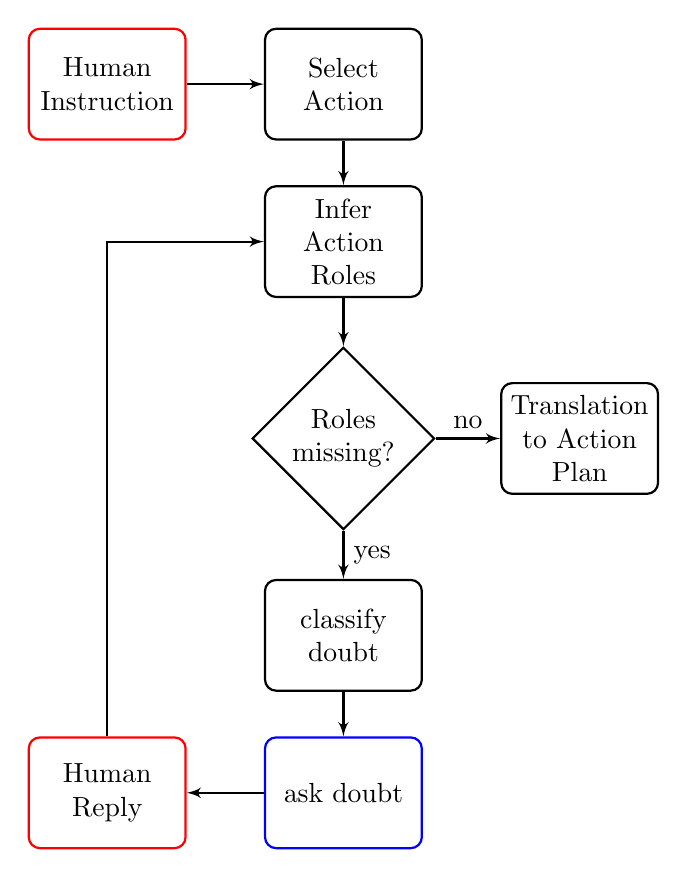
\begin{tikzpicture}[thick, scale=1,every node/.style={scale=1}, node distance= 2cm, auto]

\tikzstyle{decision} = [diamond, draw, fill=white!20, 
    text width=4.5em, text badly centered, node distance=3cm, inner sep=0pt]
\tikzstyle{block} = [rectangle, draw, fill=white!20, 
    text width=5em, text centered, rounded corners, minimum height=4em]
\tikzstyle{line} = [draw, -latex']
\tikzstyle{cloud} = [draw, ellipse,fill=gray!20, node distance=3cm,
    minimum height=2em]

    % Place nodes
    \node [block, draw=red] (hnli) {Human Instruction};
    \node [block, right of=hnli, node distance=3 cm] (aselect) {Select Action};
%    \node [cloud, left of=init] (expert) {expert};
%    \node [cloud, right of=init] (system) {system};
    \node [block, below of=aselect] (infer) {Infer Action Roles};
 %   \node [block, below of=infer] (evaluate) {evaluate candidate models};
%    \node [block, left of=evaluate, node distance=3cm] (update) {update model};
    \node [decision, below of=infer, node distance=2.5cm] (decide) {Roles missing?};
    \node [block, right of=decide, node distance=3cm] (taplan) {Translation to Action Plan};
    \node [block, below of=decide, node distance=2.5cm] (udoubt) {classify doubt};
    \node [block, below of=udoubt, draw=blue] (askdoubt) {ask doubt};
    \node [block, left of=askdoubt, node distance=3cm, draw=red] (hreply) {Human Reply};
%    \node [block, below of=decide, node distance=3cm] (stop) {stop};
    % Draw edges
    \path [line] (hreply) |- (infer);
    \path [line] (askdoubt) -- (hreply);
    \path [line] (decide) -- node{no} (taplan);
    \path [line] (decide) -- node{yes} (udoubt);
    \path [line] (aselect) -- (infer);
    \path [line] (infer) -- (decide);
    \path [line] (hnli) -- (aselect);
    \path [line] (udoubt) -- (askdoubt);
%    \path [line] (evaluate) -- (decide);
%    \path [line] (decide) -| node [near start] {yes} (update);
%    \path [line] (update) |- (infer);
%    \path [line] (decide) -- node {no}(stop);
 %   \path [line,dashed] (expert) -- (init);
 %   \path [line,dashed] (system) -- (init);
 %   \path [line,dashed] (system) |- (evaluate);
\end{tikzpicture}
\caption{A high-level flow chart of the dialog-based action role disambiguation procedure.}
\label{fig:flow}
\end{figure}    
% \vspace{3mm}
% \begin{tikzpicture}[scale=0.8,every node/.style={scale=0.8},->,>=stealth',shorten >=1pt,auto,node distance=5cm,
%                     thick]
% %  \tikzstyle{every state}=[fill=red,draw=none,text=white]
% 
%   \node[initial,state,draw=red,text=black] (A)                    {$Human$};
%   \node[state,draw=blue,text=black]         (B) [right of=A] {$Robot$};
% 
%   \path (A) edge [bend left] node {\small \sffamily \color{red} instruction (Natural Language)}  (B)
%         (B) edge [bend left, draw=gray]              node {\sffamily \small \color{blue} doubt (Controlled Natural Language)} (A);
% \end{tikzpicture}
% 
% \vspace{1mm}
Figure \ref{fig:flow} represents the interaction that can continue until the robotic assistant reaches a sufficient level of understanding. 
Taxonomical, temporal, substitution, impossibility clarifications are only some of the \textit{disambiguation cases} in which an explicit verbal task querying is necessary from the robot to the human. 
The generation of natural-like language is non-trivial given the scalability issues of linguistic factors of the sentence construction (e.g. anaphora resolution, number/gender/particle concordance, subordinate sentence handling, punctuation, verb conjugation). These requirements have proven to be fulfilled by Attempto Controlled English, now used as means of sentence construction. To do so, we make use of the ACE system's verbalization functions, used to generate ACE sentences from ontological knowledge.
Specifically for an action-oriented representation, we present our cognitive verbalization procedure, operated for each non-assigned action role:

\begin{enumerate} %TODO I don't know how to put across the following in a clearer way
    \item identification of the \textit{disambiguation cases}  (i.e. type of doubt)
    \item articulation of such doubt in a statement encapsulating what was inferred, and an interrogative sentence %to query the object itself% (to query the object itself, knowing its syntactic type) 
    \item integration of the reply, assigning the previously missing action roles 
\end{enumerate}

\subsection{Implementation} %to be improved

       
We now describe the implementation of the system by defining a pseudocode (Algorithm \ref{alg:dbard}) that incorporates references for sub-functions hereafter described (\ref{C1},\ref{C2},\ref{C3}).


\IncMargin{0.3em}
\begin{algorithm}%algopart

%\SetAlgorithmName{DisambiguationViaDialog}{DisambiguationViaDialog}{List of Heuristics}

%\caption{Dialog-based Action Role Disambiguation}
\label{alg:dbard}
\DontPrintSemicolon
\KwData{

\begin{itemize}
  \item $PRAC$, the joint probability distribution over all \\
  used class concepts given ontology knowledge,\\ formally $P\left(\mathcal{R}\times\mathcal{A}\times\mathcal{C}\,|\,\sqsubseteq,\, \preceq \right)\nonumber \enspace$.
\item $ActionDB$, a template database with all\\ ActionRoles for each ActionVerb
\end{itemize}
}
\vspace{1mm}
\KwResult{satisfactory assignment of all the ActionRoles required by the template for successful translation into action planning.}
\vspace{1mm}
\Begin{
    \textbf{wait} for $NLI$\;
    \nlset{C1} $K \longleftarrow pracInference(NLI)$ \label{C1}\;              %TODO work on this, mathematically
    $t  \longleftarrow$ single ActionVerb from $K$\;
    %Ask for actionverb if not understood
    $T \longleftarrow retrieveTemplateRoles(t,ActionDB)$\;
    $U \longleftarrow T \setminus K$ \;
    \While{$U \neq \emptyset$}{
    %    $U \longleftarrow T \setminus K$ \;
        remove item $u$ from list of $U$ with minimum syntactic relationship arity (known in template)\;
        \nlset{C2} $doubtCase$ $\longleftarrow$ $doubtCaseIdentification(u)$\label{C2}\;
        \nlset{C3}$queryType$ $\longleftarrow$ retrieve the syntactic type related to the missing role $u$\label{C3}\; %$(u,t,ActionDB)$\;
        $sDrsT$ $\longleftarrow$ $pullDrsCase(doubtCase)$\;
        $qDrsT$ $\longleftarrow$ $pullDrsCase(queryType)$\;
        $sParam$, $qParam$ $\longleftarrow$ inferred or known contextual information necessary for the grounding of specific templates of statement and question\;
        $sDrsGnd$,$qDrsGnd$ $\longleftarrow$ grounding of $sDrsT$ and $qDrsT$, via syntactic substitution of $sParam$ and $qParam$, respectively.\;% $grndDrs(sDrsT,sParam)$\;
       % $qDrsGnd$ $\longleftarrow$ $grndDrs(qDrsT,qParam)$\;
        \nlset{C4}$aceS$ $\longleftarrow$ $verbalizeDRStoACE(sDrsGnd)$\label{C4}\;
        $aceQ$ $\longleftarrow$ $verbalizeDRStoACE(qDrsGnd)$\;
        \textbf{output} aceS\;
        \textbf{output} aceQ\;
        \textbf{wait} for $reply$\;
        \nlset{C5}$N$ $\longleftarrow$ $pracInference(reply)$\label{C5}\;
        $K$ $\longleftarrow$ $K \cup N$\;
        $U \longleftarrow T \setminus K$ \;
    }
}
\caption{{Action Role Disambiguation via H-R dialog}}
\end{algorithm}
 
\paragraph{action role inference~(\ref{C1})} 
Operates an instantiation of the action template slots with the most likely class concepts, derived from the joint probability distribution of Equation \ref{pracformula}.
A lack of assignment to an action role can be due to the impossibility of 
defining a likely candidate (all probability assignments 
are below a threshold), the presence of manifold candidates
 (probability assignments are too close), or the optimal
  candidate is not available in context.
For a more formal and in-depth description of such process we
 refer to \cite{nyga12actioncore}.

\paragraph{case identification~(\ref{C2})} is operated when
 a role slot stated in our action core template has not yet been assigned for the previously described reasons.
Such abstract cases are represented in Discourse Representation Structure (DRS) templates that also encapsulate contextual information.%TODO explain better
%The following .
%This has been implemented by creating an 
%abstract DRS template for each disambiguation case, that is grounded 
%before executing the verbalization phase.
%\vspace{2mm}
\begin{figure}[H]
{\sffamily \selectfont
{\large \textsc{two-choices}}:\\
  \textbf{query\_case}: doubt between two plausible objects\\
   \textbf{template}: There is a X1, there is a X2.\\
   \textbf{drs}: drs([A,B],[object(A,X1,countable,na,eq,1)-1/4,
   object(B,X2,countable,na,eq,1)-1/9])\\
   \textbf{dependencies}: PARAM1-ext, PARAM2-ext; X1, X2\\
}
\caption{DRS template of a twofold doubt choice for a role assignment}
\end{figure}

Case identification is performed via threshold evaluation of probability values of the most likely concept candidates for the missing role.\\
More formally, let $firstMostLikely$ be: {\normalsize 
\begin{equation}
  \displaystyle \arg \max P(neededRole\ |\ knownRoles, KB\left(\sqsubseteq,\preceq\right))
\end{equation}
}
We then can describe our procedure as:\\

\vspace{2mm}
{
\Switch{$\left(P\left(firstMostLikely\right)\right)$}{
    \Case{
    is less than $possibilityThreshold$
   }
   { 
        \Return \textquotedblleft Impossibility\textquotedblright \;
    }
    \Case{is less than\\ \mbox{$P\left(secondMostLikely\right) - proximityThreshold$}
    }{
        \Return "Two-choices"\;
    }
    \vspace{2mm}
    {\LARGE $\vdots$}
    \vspace{2mm}
    
    \Other{
        \Return "None"\;
    } 
}
}
\vspace{2mm}

\paragraph{typed syntactic parsing (\ref{C3})} 

Together with a statement of the doubt case identification that encapsulates contextual information, a specific object query will also be verbalized in the form of a question. All template action roles have a 2-way relationship with a syntactic type within the scope of the action. These types are abstracted in DRS cases (same as to the DRS modeling described in \ref{C2}, e.g. in Figure \ref{drsinstr}), that need to be retrievable given the missing action role.

The knowledge regarding the association between the action roles and the syntactic type is provided by a 
\textit{controlled template}, an 
ACE sentence that comprises all uninstantiated action roles in a 
possible syntactic configuration, built upon PRAC template 
model construction (an abstraction for all instances of that action 
verb, e.g. 'flipping').
Figure \ref{ctrlst} provides an example of such modeling.
%Template Action Roles and contextual istantiation parameters of the DRS templates have a and coincide with
 %the syntactic relationships of a 
 
 \begin{figure}

{\color{gray}\footnotesize
\xytext{
  \xybarnode{\color{red} {The}} 
  &
  \xybarnode{\bf\textsc{\color{red} INSTRUMENT}}
    \xybarconnect[3][-](DL,D){-1}"^{\small det}"
    \xybarconnect[3][-](U,UL){1}"^{\small nsubj}"
  &
  \xybarnode{\bf \textsc{\color{red}FLIPS}}
    \xybarconnect[3][-](UR,U){2}"^{\small dobj}"
    \xybarconnect[10][-](U,U){4}"^{\small prep\_from}"
  &
  \xybarnode{{\color{red}the}}
    \xybarconnect[3][-](D,D){1}"^{\small det}"
  &
  \xybarnode{\bf \textsc{\color{red}THEME}} &
  \xybarnode{{\color{red}from}}
  &
  \xybarnode{\bf \textsc{\color{red}FIXEDLOCATION}}
  \xybarnode{.}
}
}
\caption{\textit{Controlled template} example for ActionVerb '\textit{flipping}'}
\label{ctrlst}
\end{figure}


The syntactic relationships in such a CNL sentence provide a formal understanding of the language-explicit relationships between the entities involved in the action. 
%This will be of use since all DRS templates will then refer to this 
%possible syntactic formulation. 
The relationships and the syntactic types from the latter 
are obtained by processing the sentence with a typed syntactic parser (for our implementation, the Stanford Parser \cite
{mcdm08b}).
%Unknown syntactic types related 
%to the missing roles are taken from the instantiated version of such 
%sentence, that comprises the known roles so far, and queried. 

\begin{figure}[H]
{\sffamily {\color{black}\large \textsc{instrumental}}:\\
\hspace{6mm}       {\color{black}\textbf{query\_case}: preposition of instrument}          \\
\hspace{3mm}       {\color{black} \textbf{template}: What X1 the X2?               }       \\
\hspace{3mm}       \textbf{drs}: drs([],[question(drs([A,B,C],[query(A,what)-1/1,         \\
\hspace{3mm}       object(C,X2,countable,na,eq,1)-1/4,                                    \\
\hspace{3mm}       predicate(B,X1,A,C)-1/2]))])                                           \\
\hspace{3mm}       {\color{black}\textbf{dependencies}: NSUBJ-left, NSUBJ-right; X1, X2 }  \\
%The system has proved scalability given also the aggregation capability of DRS.
\caption{DRS template of an 'instrument' object query}
\label{drsinstr}
}
\end{figure}
%Stress on verbalization functions.
\paragraph{sentence construction (\ref{C4})} is to provide a grammatical structure for the grounded discourse abstractions of the case identification statement and the object query question. This is implemented by using the ACE verbalizer functions, providing grounded DRS instances as a formal parameter.   

The approach of verbalization of two phrases, namely doubt statement and object question has been chosen to provide the human with a better understanding of both the uncertainty (e.g. "what instrument should be used?") and of what has been inferred (e.g. doubt between spatula or tongs). 

\paragraph{reply integration (\ref{C5})} is performed by making use of the previously described action role inference routine on the natural language reply. After retrieving the new action role assignments, we will substitute in the main instance only the newly identified action 
roles that were previously missing. The pipeline
of reasoning is shown with an example in Figure \ref{fig:pipeline}.

%\vspace{3mm} %TO BE INTEGRATED
%{\sffamily
% To be asked:\\
%   - Ask for missing role \textbf{"Instrument"},\\ 
%     case \textbf{"two-choices"}\\
%   - Ask for missing role \textbf{"Instrument"},\\
%     case \textbf{"nsubj"}  \\
% \textbf{\color{red}\\
% Verbalization: \\
% ACE: [[There is a spatula.],[There is a n:tongs.]]\\
% ACE: [[What v:flips a pancake?]]\\
% }
% }

%The DRS templates are instantiated by substituting 
%syntactically contextual information taken from the initial Natural 
%Language Instruction, or from the inferred probability distribution 
%of likely objects (i.e. dependencies). This is then verbalized with 
%the DRS$\Rightarrow$ACE verbalizer module, process that accounts for 
%the linguistic issues described beforehand.\\ Having stated the 
%nature of the ambiguity (e.g. comparison, impossibility) the 
%abstract case is followed by a question asking the object, 
%given the syntactic type (e.g. instrument, direct object, 
%preposition from/to). The verbalization process for the latter 
%follows the same procedure stated for the disambiguation cases. \\ 


%The querying procedure is identical to the one above, via the use of 
%similar templates.

\begin{figure}[t]
\centering
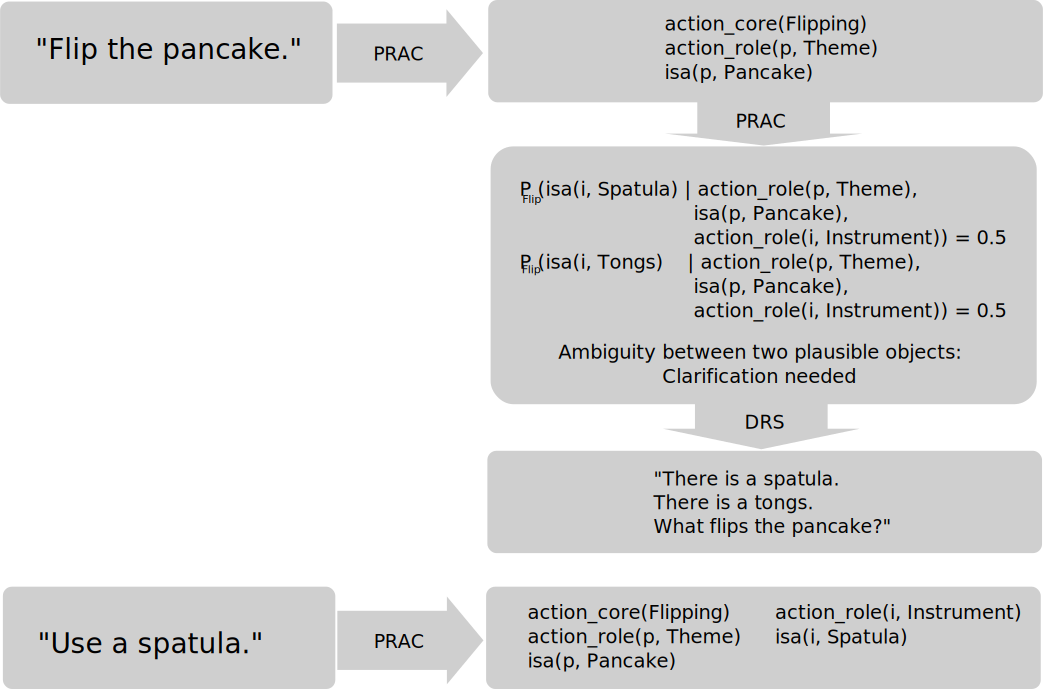
\includegraphics[width=1\columnwidth]{results.pdf}
\caption{Reasoning pipeline of a possible instance of disambiguation interaction}
\label{fig:pipeline}
\end{figure} 

\section{CNL for Action Formalization}
For the formalization of a PRAC model, be it grounded or abstract, we 
require a format that can serialize the instance or generate the PRAC 
model template.
We therefore need a statement that comprises all generative information,
 namely all roles involved in the action, and the data that can create 
 the MLN formulas that evaluate the probability of all possible syntactic 
types the action roles can be involved in.

We create this by encapsulating the action roles as nouns in a Controlled 
Natural Language statement, for human-readability and for preserving the 
syntactic relationships between the objects; furthermore we add explicit 
semantic tags to maintain information regarding semantic disambiguation
 of objects.
An implementation is possible via the use of ACE and semantic tags from 
WordNet\cite{Miller95wordnet:a}. To pursue the example of above:
\vspace{3mm}

{\sffamily
The AGENT.n.06 FLIPS.v.08 the THEME.n.01 
from LOCATION.n.01 with an INSTRUMENT.n.01. 
}$^1$\\

\vspace{2mm}
An example of the semantic information that is then retrievable:\\
\vspace{2mm}

{\small
{\sffamily
\textbf{agent.n.06} {\color{red}(the semantic role of the animate entity 
that instigates or causes the happening 
denoted by the verb in the clause)}}
}
\vspace{2mm}

\paragraph{template generation} will create, given $^1$, 
an initial set of action roles and MLN formula templates.  
The action roles correspond to the nouns of the generating sentence, 
and their type of syntactic relationship defines the variant MLN 
templates. Other lexicographical 
information such as descriptions can be retrieved via preexisting 
webservices.

\section{Results, Discussions and Conclusions}
This paper brings attention to possible uses of Controlled Natural 
Languages in the artificial cognition domain. While already proven 
as powerful means of representation and reasoning for the semantic 
web\cite{kaljurandphd}, our claim is that novel uses are possible 
for robotic assistants, specifically as human-to-robot interface.
We have proven via practical implementations that CNL can be exploited
 as means of language generation and presented current work in progress
  in relation to full action-oriented cognitive formalization.

However, even if it is an easier instrument for achieving knowledge 
engineering, CNL construction is not always straightforward \cite
{Schwitter05alayered}. In fact, the DRS construction of the 
disambiguation cases had to account for the ACE construction rules 
(that can present expressiveness limitations) and the asymmetry of 
what is accepted as correct ACE statement and what can be verbalized 
(e.g. modals). The verbalizer system being purely a DRS and PRAC 
based syntactical manipulator, is constrained by the current 
implemented features of these and presents similar limitations. This 
is visible since the verbalization outputs are readable but not 
perfectly natural-like sentences, and on the other hand we have 
scalability issues given by improper object probability inference. 
With the expansion of the expressiveness set of ACE and DRS, 
future work will aim towards how 
to make use of such abstractions in order to provide robotic 
assistants with further means of expression. 
In reference to action formalization, the practical implementation 
of a PRAC model template generator will provide insights regarding
 representation limitations, for now discussed only theoretically. 
Further research will 
also be dedicated to the interaction dialogue itself and to \textit
{learning via human-robot verbal interaction}, made possible via 
template generation and further knowledge manipulation, thanks to 
the common ground of Controlled Natural Languages.


%\addtolength{\textheight}{-12cm}   % This command serves to balance the column lengths
                                  % on the last page of the document manually. It shortens
                                  % the textheight of the last page by a suitable amount.
                                  % This command does not take effect until the next page
                                  % so it should come on the page before the last. Make
                                  % sure that you do not shorten the textheight too much.


\section*{Acknowledgments}
This work has been partially supported by the EU FP7 Projects
\emph{RoboHow} (grant number 288533) and \emph{ACAT} (grant number 600578).


\bibliography{bibform}{}
\bibliographystyle{IEEEtran}

\end{document}
